%!TEX encoding = UTF-8 Unicode
% coding: utf-8

%!TEX encoding = UTF-8 Unicode
% coding: utf-8
% Header per le presentazioni in LaTeX+beamer
% @author Eric Miotto
% @date 15/12/2006

\documentclass{beamer}

%Configurazione beamer
\mode<presentation>
{
 %Tema grafico
  \usetheme{Frankfurt}
  
  %Colori da usare per il tema
  \usecolortheme{seahorse} 
  \usecolortheme{rose} 

  \setbeamercovered{transparent}
}

%Importazione package
\usepackage[italian]{babel} %Lingua e sillabazione in italiano
\usepackage[utf8]{inputenc} %Codifica UTF8
\usepackage{textpos} %Posizionamento testo e immagini ovunque sulla pagina

% Griglia di posizionamento delle immagini
% Il primo parametro sono il numero di colonne in cui viene diviso il foglio,
% il secondo sono il numero di righe in cui viene diviso il foglio
%\TPGrid{3}{1}

\title{Presentazione Definizione di Prodotto \\ per C04}

\author{Egoless Group}

\date[RPD 28/02/2007] % (optional, should be abbreviation of conference name)
{Revisione di Progetto Definitivo \\ 28 febbraio 2007}

\subject{Presentazione della definizione di prodotto per il capitolato C04}

\logo{
\includegraphics[width=1cm]{img/logo.jpg}}

% Delete this, if you do not want the table of contents to pop up at
% the beginning of each subsection:

%Ci pensa lui a creare l'indice

\AtBeginSubsection[]
{
  \begin{frame}<beamer>
    \frametitle{Outline}
    \tableofcontents[currentsection,currentsubsection]
  \end{frame}
}

%\AtBeginSection[]
%{
%  \begin{frame}<beamer>
%    \frametitle{Outline}
%    \tableofcontents[currentsection]
%  \end{frame}
%}

\begin{document}

\begin{frame}
  \titlepage
\end{frame}

\begin{frame}
  \frametitle{Outline}
  \tableofcontents
  % You might wish to add the option [pausesections]
\end{frame}


% Structuring a talk is a difficult task and the following structure
% may not be suitable. Here are some rules that apply for this
% solution: 

% - Exactly two or three sections (other than the summary).
% - At *most* three subsections per section.
% - Talk about 30s to 2min per frame. So there should be between about
%   15 and 30 frames, all told.

% - A conference audience is likely to know very little of what you
%   are going to talk about. So *simplify*!
% - In a 20min talk, getting the main ideas across is hard
%   enough. Leave out details, even if it means being less precise than
%   you think necessary.
% - If you omit details that are vital to the proof/implementation,
%   just say so once. Everybody will be happy with that.

\section{Pianificazione}

\subsection*{Pianificazione}

\begin{frame}
\frametitle{Pianificazione}

\begin{itemize}
\item le ore erogate sono molto di più di quelle previste
\item di conseguenza la pianificazione è slittata in avanti
\item stiamo lavorando per ripianificare in maniera adeguata
\end{itemize}

\end{frame}

\section{Definizione di Prodotto}

% Trucco per far apparire i pallini per ogni slide
% Bisogna sempre creare una sottosezione,
% ma con il comando \subsection* (con l'asterisco)
% In questo modo la sottosezione non
% figura nella TOC, ma i pallini vengono visualizzati lo stesso
% Per convenzione (temporanea) do' alla sottosezione lo stesso titolo
% della sezione (potrebbe essere anche vuoto).
\subsection*{Presentiamo di nuovo l'architettura}
%\subsection*{}

\begin{frame}
\frametitle{Architettura generale}

\begin{center}
  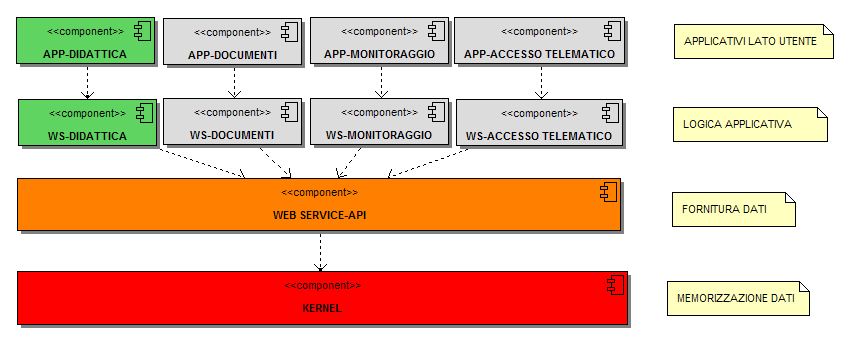
\includegraphics[width=12cm]{../../immagini/ArchitetturaGenerale.png}
\end{center}
\end{frame}

\subsection{WS Didattica}

\begin{frame}
\frametitle{Tecnologie usate per l'implementazione}

\begin{itemize}
\item Java Enterprise Edition 5, in particolare

\begin{itemize}
\item Glassfish, application server Java EE
\item JAX WS 2.0 per creare il Web Service
\end{itemize}

\end{itemize}

\end{frame}

\begin{frame}
\frametitle{Dettaglio di WS Didattica}

\begin{itemize}
\item classi generate da JAX WS per comunicare con WEB SERVICE API
\item classe Enterprise JavaBean che implementa la logica di WS Didattica
\item ogni metodo esposto allo strato applicativo lancia un'eccezione quando si verificano errori
\end{itemize}


\end{frame}

\subsection{APP Didattica}

\begin{frame}
\frametitle{Tecnologie usate}

\begin{itemize}
\item Java 5, in particolare

\begin{itemize}
\item Swing
\item JavaBean
\item \ldots tutto con l'ausilio di NetBeans 5.5 con Enterprise Pack
\end{itemize}

\end{itemize}
\end{frame}

\begin{frame}
\frametitle{Dettaglio di APP Didattica}

\begin{itemize}
\item Applicazione strutturata secondo il pattern architetturale MVC
\item ogni classe da manipolare viene gestita da un modello implementato usando JavaBean:
\begin{itemize}
 \item recuperare oggetti dal Web Service sottostante
 \item permettere l'accesso e/o modifica delle proprietà dell'oggetto
 \item notificare le modifiche a tutte le View in ascolto (\ldots pattern Observer)
\end{itemize}

\item l'interfaccia grafica in Swing fa contemporaneamente da View e da Controller
\end{itemize}

\end{frame}


\section{Evoluzione del Piano di Qualifica}

\subsection*{Evoluzione del Piano di Qualifica}

\begin{frame}
\frametitle{Evoluzione del Piano di Qualifica}

\begin{itemize}
	\item Definizione dell'infrastuttura tecnologica
	\begin{itemize}
		\item Strumenti di test
		\item Strumenti di analisi statica
		\item Tool per il tracciamento
	\end{itemize}
	\item Adozione di metriche
	\begin{itemize}
		\item per la progettazione
		\item per la codifica
	\end{itemize}
\end{itemize}

\end{frame}

\begin{frame}
\frametitle{Definizione dell'infrastruttura tecnologica}
\framesubtitle{Strumenti di analisi}
\begin{itemize}
	\item Strumenti di test
	\begin{itemize}
		\item \alert{JUnit} per il test funzionale
		\item \alert{Cobertura} per la verifica di branch e statement coverage
	\end{itemize}
	\item Strumenti di analisi statica
	\begin{itemize}
		\item \alert{FindBugs} per ricerca di bug patterns
	\end{itemize}
	\item altri (ricerca in corso)
\end{itemize}
\end{frame}

\begin{frame}
\frametitle{Definizione dell'infrastruttura tecnologica}
\framesubtitle{Tool per il tracciamento}
\begin{itemize}
	\item utilizzeremo OSRMT (www.osrmt.com)
	\item infrastruttura semplice da creare (file database condiviso con svn)
	\item rapido da introdurre
	\begin{itemize}
\item 2 ore per studiare il tool
\item 2 ore per introdurre i dati
\end{itemize}

\end{itemize}
\end{frame}

\begin{frame}
\frametitle{Metriche adottate}
\begin{itemize}
	\item Fan-in e Fan-out
	\begin{itemize}
		\item Cercheremo un tool per la misurazione automatica
	\end{itemize}
	\item SLOC 
	\begin{itemize}
		\item porre (eventualmente) limiti alla lunghezza dei metodi o dei file
	\end{itemize}
	\item Complessità ciclomatica
	\begin{itemize}
		\item Posti dei limiti iniziali, da adattare se necessario
		\item Misurata automaticamente (Cobertura)
	\end{itemize}
	\item Altre in fase di studio (Function Point, ...)
\end{itemize}
\end{frame}


\section{Cosa abbiamo sbagliato finora}

\subsection*{Cosa abbiamo sbagliato finora}

\begin{frame}
\frametitle{Cosa abbiamo sbagliato finora}

\begin{itemize}
\item pianificazione
\begin{itemize}
	\item aumento del numero di ore progettazione per acquisire padronanza delle tecnologie adottate
\end{itemize}
\item adottato BoUML al posto di ArgoUML
\begin{itemize}
	\item supporto a UML 2.0
	\item meno user-friendly ma più completo
\end{itemize}
\item collaborazione in fase di assestamento
\end{itemize}

\end{frame}

\end{document}